\documentclass[a4paper,12pt]{article}
\usepackage[utf8]{inputenc}
\usepackage[T2A]{fontenc}
%\usepackage[russian]{babel}
%\usepackage{fullpage}
\usepackage{graphicx}
\graphicspath{{../}}
\usepackage{setspace}
\usepackage{hyperref}
\hypersetup{
    colorlinks=true,
    linkcolor=blue,
    filecolor=magenta,      
    urlcolor=cyan,
}
\textwidth=18cm \textheight=25cm \oddsidemargin=-10mm \topmargin=-3mm
\headheight=-12mm \headsep=10mm
\parindent=1.2cm
\renewcommand{\baselinestretch}{1.25}

%148×210 мм

\begin{document}
\renewcommand{\baselinestretch}{1.3}\selectfont
%✂---------------------------------------------------
\pagestyle{empty}
{
\huge
\begin{center}
A short report on a test task of PROSAIL RTM use for different grasslands
\end{center}
}

\vspace{5mm}

The task was \textit{to set-up a rough framework which simulates the reflections of 2 grassland types (extensive \& intensive use) at 3 points within the vegetation period (spring, summer, autumn). Please use the PROSAIL applications of your preferred language (R, matlab, Python \ldots)}.

My vision of it was the following:
\begin{itemize}
	\item obtain GRASSMIND and PROSAIL models;
	\item try to run them separately and take a look at the inputs and outputs;
	\item check if I can configure the GRASSMIND model to imitate the proposed setup, i.e. intensive and extensive grasslands during different seasons;
	\item use PROSAIL model with the inputs from the GRASSMIND or prepare six sets of values for input parameters for it;
	\item analyse the results.
\end{itemize}

Since the aim is to meld GRASSMIND and PROSAIL, the first one should provide some inputs for the last. Quick literature scan revealed that there is LAI value among the GRASSMIND outputs which is needed for PROSAIL. 

\begin{center}
	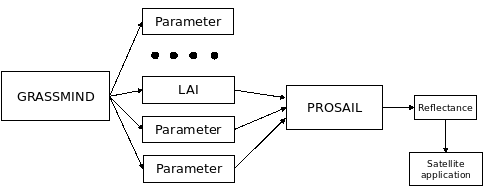
\includegraphics[width=0.8\linewidth]{../figs/Diagram1.png} \\
\end{center}

However, the model won't run after compilation: trying to start any on the test cases (\textit{Mixture\_Poa\_Plantago, Monoculture\_Fpratensis, Monoculture\_Planceolata, Monoculture\_Ppratensis}) resulted in crash with: \pagebreak

\begin{verbatim}
ERROR: Field capacity (FC) is partly smaller than permanent wilting point (PWP) 
in soil file but should always be bigger . 
File: /home/miakunin/iDiv/Interview_1/GRASSMIND/SourceCode/for_environment.cpp  
Line: 1204
Aborted (core dumped)
\end{verbatim}

I checked the soil input files and found that $FC$ values were always set higher than $PWP$, however:
\begin{verbatim}
Layer	RWC[-]	FC[V%]	PWP[V%]	MineralN[gm-2]		
1	0.0	27.6	14.3	0.12
2	0.5	28.0	14.9	0.45
3	1.0	28.0	14.9	3.73  
\end{verbatim}

Having no other clue I decided to focus on PROSAIL "stand-alone". I obtained the source code from \url{http://teledetection.ipgp.jussieu.fr/prosail/} choosing \textit{PROSAIL\_5B\_Fortran} version since I am more familiar with FORTRAN.

The model runs fast and writes reflectance with 1 nm step to the ASCII output file. All the input parameters are hardcoded in the main, so I reworked it a little to improve utility and make the model read some principal input values from a standard FORTRAN namelist file.

For the test case the following parameters was chosen: \textit{LAI, Cab, Car, Cbrown, Cw, Cm, N, hsop, psoil.} An abundance of literature where PROSAIL model was used revealed possible ranges for the variables, and I ended up with the following for the test cases:

\begin{center}
\begin{tabular}{ l | l l l | l l l }
~	&  \multicolumn{3}{|c|}{Extensive} & \multicolumn{3}{|c}{Intensive}		\\
~	&Spring	&Summer	&Autumn	&Spring	&Summer	&Autumn \\
\hline
LAI	&2.5 	&6	&3.5 	& 3	&8	&6 \\
Cab	&20	&30&	25	&20	&50	& 35 \\
Car	&6	&7	&8	&6	&7	&8 \\
Cbrown	&0	&0.05	&0.2 &	0	&0	& 0.1\\
Cw	& 0.02	&0.02 &	0.01 &	0.02 &	0.03 &	0.02 \\
Cm	&0.005	& 0.005	&0.01	&0.005	&0.005	&0.007 \\
N	&1.5	 &1.5 &	1.5	& 1.5	& 1.5	& 1.5 \\
hsop &	0.01 &	0.01 &	0.01 &	0.01 &	0.01 &	0.01 \\
psoil &	0.1	&1	&0.2 &	0.1	&0.1 &	0.2 \\
\end{tabular}
\end{center}

For the leaf slope I used default values from the model code and the Sun geometry was 30$^{\circ}$ solar zenith angle, 10$^{\circ}$  observer zenith angle, and 0$^{\circ}$ for the azimuth. The result of the model is shown in the following figure:\footnote{All the analysis I'll leave for the online discussion}

\begin{center}
	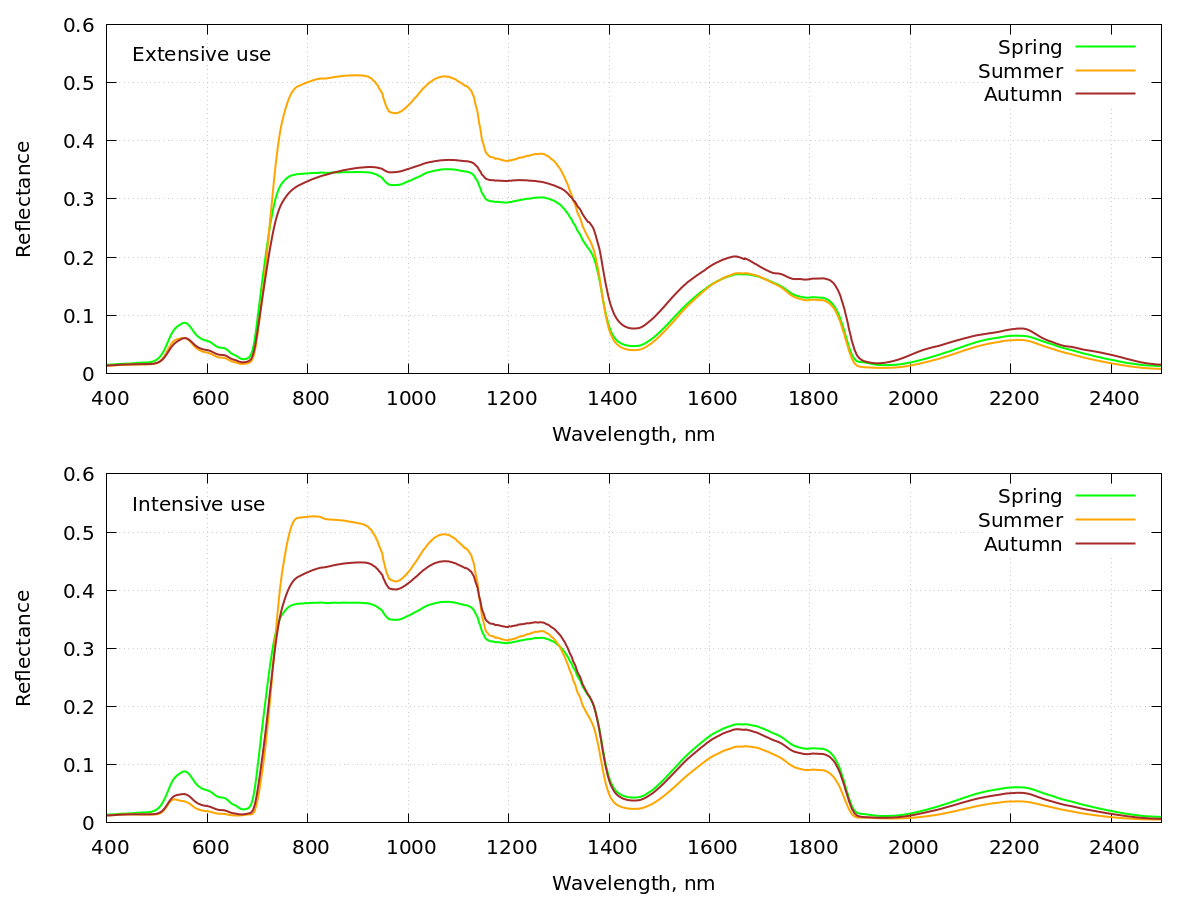
\includegraphics[width=0.7\linewidth]{../plt/intensive-extensive_grasslands.png} \\
\end{center}

Then, following the work of Imran et al., (VIS-NIR, Red-Edge and NIR-Shoulder Based Normalized Vegetation Indices Response to Co-Varying Leaf and Canopy Structural Traits in Heterogeneous Grasslands, Remote Sens. 2020, \url{https://doi.org/10.3390/rs12142254}) I decided to run several sensitivity test for the PROSAIL model (see Fig. below).

\begin{center}
	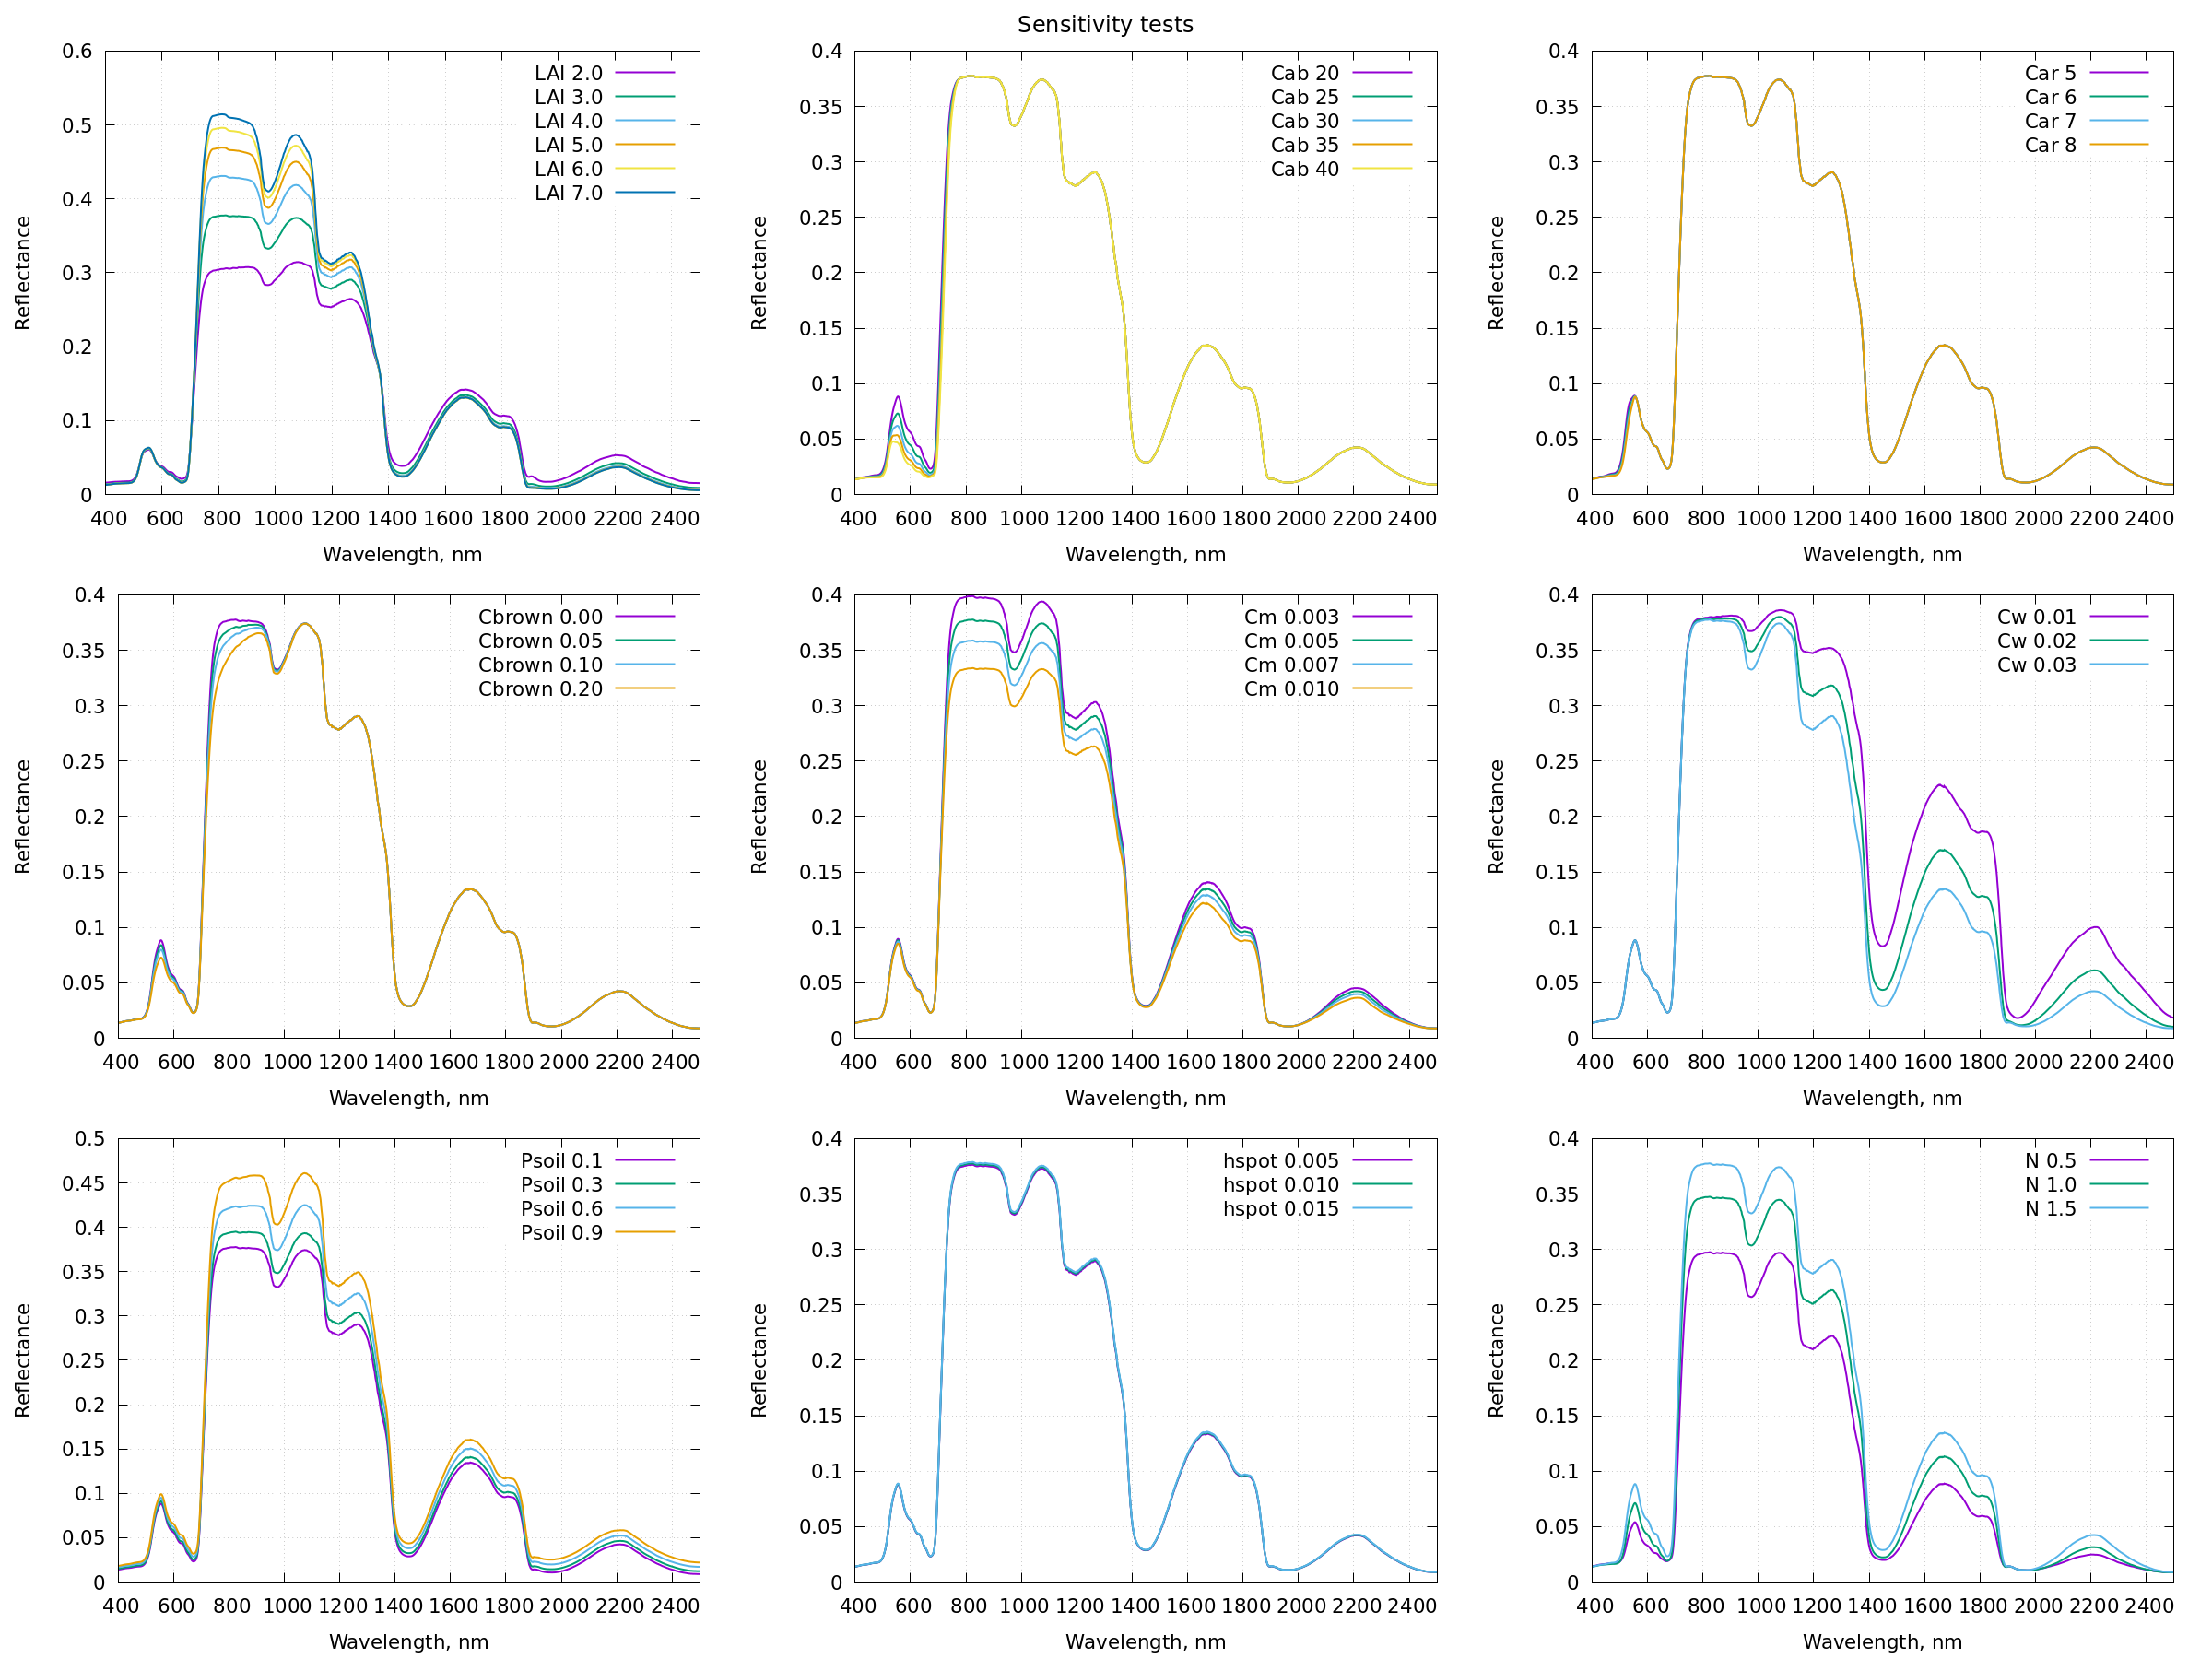
\includegraphics[width=0.9\linewidth]{../plt/sensitivity_tests.png} \\
\end{center}

\textit{Where potential differences in your simulations may stem from?} 
In the "errors" or uncertainties of the input parameters, especially from LAI, leaf thickness LMA, equivalent water thickness EWT (600 nm and more). Soil wetness is an important parameter too, and structure coefficient (N), but I don't think it could change fast.

\textit{How could GRASSMIND be used to answer these questions?} 
GRASSMIND model, as I believe, can provide actual values for required parameters, therefore reducing possible errors in the situations where in-situ measurements aren't possible.

~ \\

The tweak for the PROSAIL model is available here:\\ \url{https://github.com/miakunin/Prosail_iDiv_test.git}

PLEASE NOTE(!!) that this git provides ONLY the main file of the PROSAIL model(!!!). To compile and run it one need to get the original model files from official source: \url{http://teledetection.ipgp.jussieu.fr/prosail/PROSAIL_5B_Fortran.rar}

This was done not to violate original licenses.


\end{document}